\iffalse
It's unfair to say that mathematicians aren't real doctors, we perform surgeries all the time. In this class we'll introduce the notion of a topological manifold via simplicial (delta) complexes. Spend a day or two doing examples and go over several notions like orientation, cobordism and of course surgery.

Keywords: simplicial complex, manifold, orientation, cobordism, surgery

Type: Lecture
Homework: Recommended
Prereqs: None
\fi




\documentclass{article}
\usepackage{amsmath, amsthm}
\usepackage{amssymb}
\usepackage{mathtools}
\usepackage[all,cmtip]{xy}
\usepackage{color}


\setcounter{tocdepth}{4}

\renewenvironment{proof}{ {\bfseries Proof:}}{\qed}

\newtheoremstyle{mytheorem}%                % Name
{}%                                     % Space above
{}%                                     % Space below
{\itshape}%                                     % Body font
{0pt}%\parindent}%                                     % Indent amount
{\bfseries}%                            % Theorem head font
{.}%                                    % Punctuation after theorem head
{ }%                                    % Space after theorem head, ' ', or \newline
{}%                                     % Theorem head spec (can be left empty, meaning `normal')

\theoremstyle{mytheorem}
\newtheorem{thm}{Theorem}[section]
\newtheorem{proposition}[thm]{Proposition}
\newtheorem{lemma}[thm]{Lemma}
\newtheorem{corollary}[thm]{Corollary}


\newtheoremstyle{mydefinition}%                % Name
{}%                                     % Space above
{}%                                     % Space below
{}%                                     % Body font
{0pt}%\parindent}%                                     % Indent amount
{\bfseries}%                            % Theorem head font
{.}%                                    % Punctuation after theorem head
{ }%                                    % Space after theorem head, ' ', or \newline
{}%                                     % Theorem head spec (can be left empty, meaning `normal')

\theoremstyle{mydefinition}
\newtheorem{definition}[thm]{Definition}
\newtheorem{example}[thm]{Example}
\newtheorem{exercise}[thm]{Exercise}
\newtheorem{remark}[thm]{Remark}
%\newtheorem{ques}[thm]{Q.}
\newtheorem*{ques}{Question}
%\newtheorem{ans}[thm]{Ans.}
\newtheorem*{ans}{Ans}



\numberwithin{equation}{section}

%Real numbers, complex numbers, etc.
\newcommand{\R}{\mathbb{R}}
\newcommand{\C}{\mathbb{C}}
\newcommand{\Z}{\mathbb{Z}}
\newcommand{\Q}{\mathbb{Q}}
\renewcommand{\P}{\mathbb{P}}

%How does latex not have these?
\DeclareMathOperator{\Ad}{Ad}
\DeclareMathOperator{\ad}{ad}
\DeclareMathOperator{\tr}{tr}
\DeclareMathOperator{\Tr}{Tr}
\DeclareMathOperator{\Hom}{Hom}
\DeclareMathOperator{\Spec}{Spec}
\DeclareMathOperator{\im}{im}
\DeclareMathOperator{\rank}{rank}
\DeclareMathOperator{\Exists}{\exists}
\DeclareMathOperator{\Forall}{\forall}

\DeclareMathOperator*{\colim}{colim}
\DeclareMathOperator*{\holim}{holim}
\DeclareMathOperator*{\hocolim}{hocolim}


%fractions and inner product
\newcommand{\pr}[2][\:]{\frac{\partial #1}{\partial #2}}
\newcommand{\innerp}[2]{\langle #1, #2 \rangle}

\newcommand*\conj[1]{\overline{#1}}
\newcommand*\norm[1]{\lVert #1 \rVert}

\renewcommand{\figurename}{Fig.}
\usepackage{float}
\usepackage{wrapfig}

\usepackage{enumitem}
\setlist[enumerate]{itemsep=0mm}
\usepackage{geometry}
\geometry{
	a4paper,
	total={170mm,257mm},
	left=20mm,
	top=20mm
}


\usepackage{fancyhdr}
\pagestyle{fancy}
\lhead{\scshape Apurva Nakade}
%\rhead{\scshape Mathcamp 2017}
\renewcommand*{\thepage}{\small\arabic{page}}

\rhead{\scshape Mathcamp 2017 : All things Manifoldy}
\begin{document}
\title{Heegard splittings of 3 manifolds}
\author{Apurva Nakade}
\thispagestyle{fancy}
\maketitle


It is difficult to imagine 3 dimensional manifolds as they require at least 4 dimensions to be embedded in. Instead we describe 3 dimensional manifolds using ``gluing diagrams'' which are obtained by gluing sides of solid polytopes in 3 dimensions.

\section{The three dimensional sphere $S^3$}
The 3 dimensional sphere is defined as $$S^3 = \{ (x,y,z,t) : x^2 + y^2 + z ^{2} + t ^{2} = 1  \}$$ If we consider the standard sphere $S^2$ of radius 1 and intersect it by a vertical plane $z = c$ we get an $S^1$ if $-1 < c < 1 $, a point if $c = \pm 1$ and an empty set otherwise. Similarly if we intersect $S^3$ with $t=c$ we get a sphere $S^2$ if $ -1 < c < 1$, a point if $c=1$ and an empty set otherwise.

\begin{figure}[H]
	\centering
	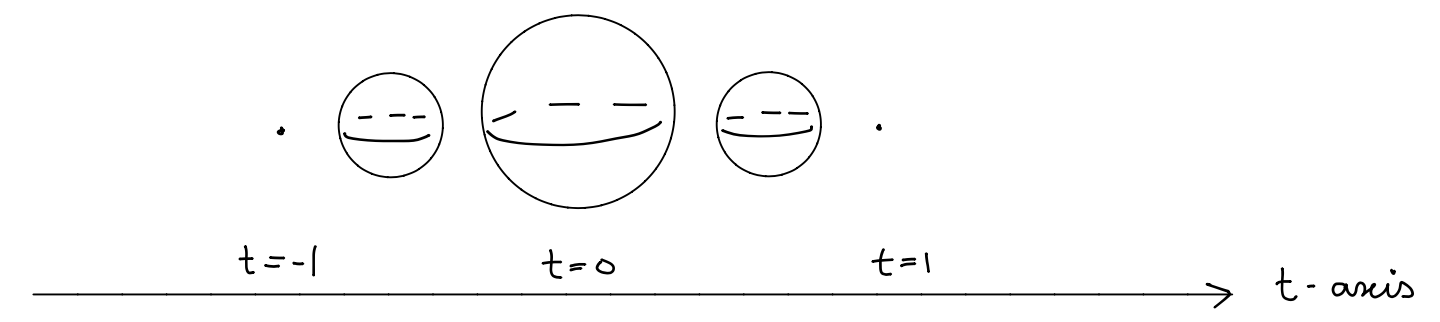
\includegraphics[width=0.90\linewidth]{../images/SphereTime}
	\caption{$S^3$ as a sequence of spheres}
\end{figure}


Another way to visualize $S^3$ is by noticing that if we remove one point from $S^3$ we get the space $\R^3$. Conversely this implies that $S^3$ is the one point compactification of $\R^3$ i.e. $S^3 = \R^3 \cup \{ *\}$.


\subsection{Hemispheres and solid tori}
Consider the two hemispheres
\begin{align*}
	S^3_+ & = \{ (x,y,z,t) : x^2 + y^2 + z ^{2} + t ^{2} = 1 , t \ge 0 \} \\
	S^3_- & = \{ (x,y,z,t) : x^2 + y^2 + z ^{2} + t ^{2} = 1 , t \le 0 \}
\end{align*}
Both $S^3_+$ and $S^3_-$ are homeomorphic to the three disc
\begin{align*}
	D^3 & = \{ (x,y,z) : x^2 + y^2 + z ^{2} \le 1
\end{align*}
via the projection maps $S^3_+ \rightarrow D^3$ and $S^3_- \rightarrow D^3$. Hence we can think of $S^3$ as two 3 dimensional discs being glued together along the boundary.

\begin{figure}[H]
	\centering
	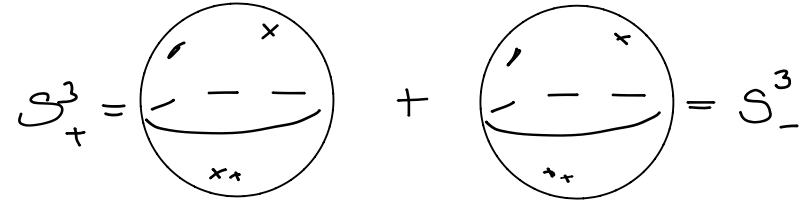
\includegraphics[width=0.5\linewidth]{../images/SphereDiscs}
	\caption{$S^3$ as two 3 discs $S^3_+$, $S^3_-$ glued together}
\end{figure}

We can perform surgery on $S^3_+$ and $S^3_-$ by removing and adding a solid cylinder respectively.
\begin{figure}[H]
	\centering
	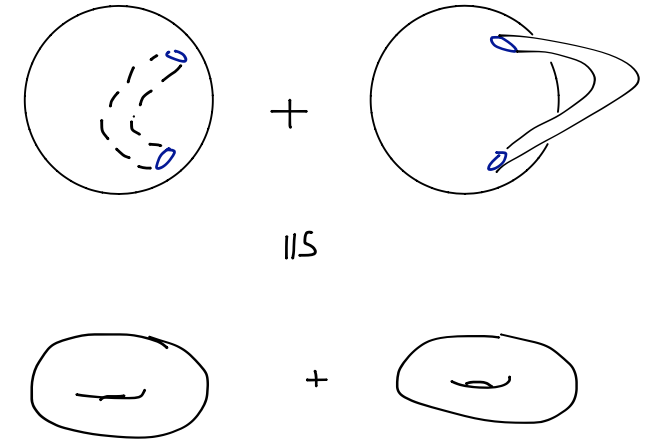
\includegraphics[width=0.25\linewidth]{../images/HeegardSphere}
	\caption{$S^3$ as two solid tori glued together}
\end{figure}

We can also remove and add multiple solid cylinders to get
\begin{figure}[H]
	\centering
	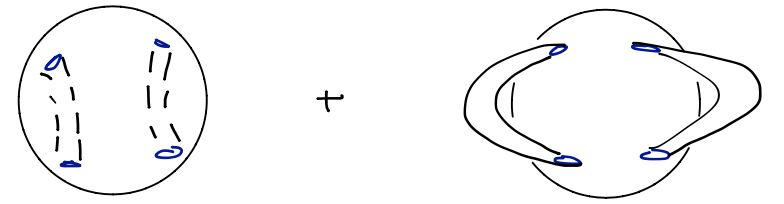
\includegraphics[width=0.25\linewidth]{../images/HeegardSphere2}
	\caption{$S^3$ as two solid genus $2$ surfaces glued together}
\end{figure}

These are called Heegard splittings of $S^3$.

\subsection{Heegard splittings of 3 manifolds}
Let $M$ be a 3 manifold and suppose we have a ``gluing diagram'' of $M$ consisting of multiple polytopes. However unlike for 2 manifolds, we do not allow different sides of the same polytope to be glued to each other.

For example, $S^3$ has a gluing diagram consisting of two solid cubes with corresponding sides glued.
\begin{figure}[H]
	\centering
	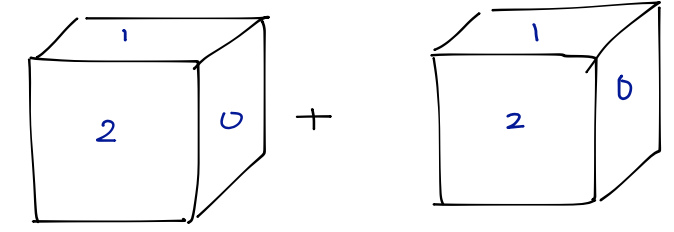
\includegraphics[width=0.25\linewidth]{../images/SphereGluingDiagram}
	\caption{$S^3$ as a sum of two solid cubes}
\end{figure}


Let $X$ be the set of edges of gluing diagram which have been thickened. And let $Y$ be the complement of $X$ in $S^3$, $Y = S^3 \setminus X$.
\begin{figure}[H]
	\centering
	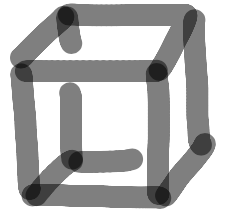
\includegraphics[width=0.15\linewidth]{../images/Heegard1}
	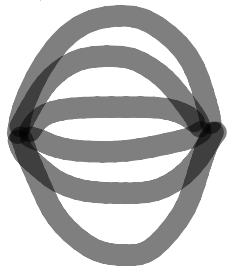
\includegraphics[width=0.15\linewidth]{../images/Heegard2}
	\caption{Heegard splitting of $S^3$, both $X$ and $Y$ are solid genus 5 surfaces.}
\end{figure}

It is not hard to see that both $X$ and $Y$ are solid surfaces of the same genus. This shows that every 3 dimensional manifold $M$ which has a ``gluing diagram'' can be obtained by gluing two solid surfaces of the same genus. This is called the \textbf{Heegard splitting} of the manifold $M$.

\section{Exercises}

\begin{exercise}
	Construct ``gluing diagrams'' for $T \times S^1$ and $S^2 \times S^1	$ using the gluing diagram of $T$ and $S^2$ and thinking of $S^1$ as two endpoints of $[0,1]$ glued together.
\end{exercise}

\begin{exercise}
	Construct Heegard splittings for $T \times S^1$ and $S^2 \times S^1$.
\end{exercise}

\begin{exercise}
	Why does this procedure not work for two dimensional manifolds?
\end{exercise}



\end{document}
